\documentclass[]{article}

\usepackage{hyperref}
\usepackage{microtype}
\usepackage{float}
\usepackage{graphicx}
\usepackage{t1enc}
\usepackage[utf8]{inputenc}
\usepackage{anysize}
\usepackage[hungarian]{babel}
\usepackage{setspace}  % Ettol a tablazatok, abrak, labjegyzetek maradnak 1-es sorkozzel!

\marginsize{20mm}{25mm}{15mm}{15mm} % anysize package

\title{\texttt{23\_14} Web Scraper}
\author{boa (\texttt{boaboa})}

\begin{document}

\maketitle

\begin{abstract}

%Write a program that extracts and aggregates news headlines from various sources.
%With Copilot, you can get help on understanding various web scraping techniques and libraries.

Egy olyan backend szoftvert fejlesztettem ChatGPT alkalmazásával, ami képes egy konfigurációs fájl alapján rss/atom folyamok szerint letölteni híreket. Mindezt még kiegészítettem azzal, hogy az alap feed-ben megtalálható adatok mellett a cikk teljes szövegét is leszedi. A cikk szövegéhez az url-en található html dokumentumot értelmezi a program, szintén a konfigurációs fájl szerint. A híreket el is tárolja a szoftver és egy API-on elérhetővé teszi JSON formátumban. Grafikus kezelői felület helyett arra koncentráltam, hogy sok hírportált támogasson a program.

\end{abstract}

\pagebreak

\section{Tervezés}

A ChatGPT promptolásánál mindig angol nyelvű szöveget használtam, mert abban jobb a modell (lévén, hogy tanítás közben abból többet látott).

\begin{figure}[H]
	\centering
	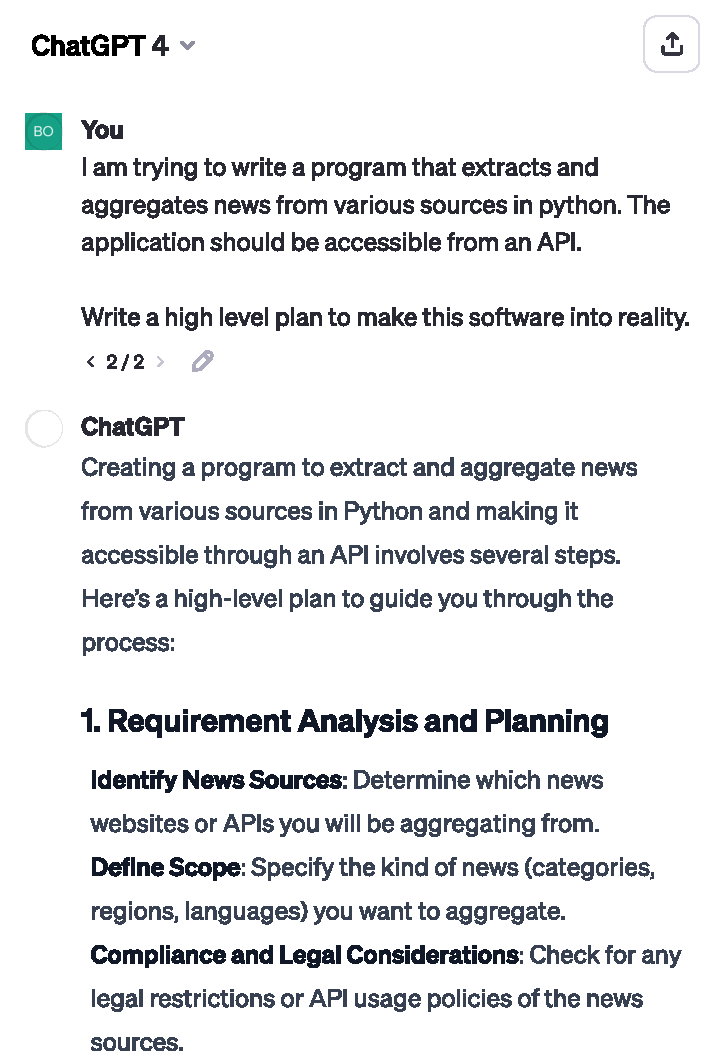
\includegraphics[width=0.7\textwidth]{prompt_1.pdf}
	\caption{Kezdeti prompt (nem teljes válasz)}
\end{figure}

A ChatGPT kimenetét megvizsgálva és saját tudásomra támaszkodva úgy döntöttem RSS/Atom folyamok periódikus letöltésével fogom az új híreket megszerezni. A teljes szöveghez viszont általában csak a cikket tartalmazó oldal letöltése és értelmezése után lehet hozzáférni, erre \texttt{Beautiful Soup} Python könyvtárat választottam. Az adatok eltárolását az egyszerűség kedvéért egy lokális Sqlite adatbázissal oldottam meg. Végül pedig az adatokat \texttt{FastApi} python könyvtár segítségével tettem elérhetővé egy API endpointon.

\section{Megoldás}

\subsection{Alapok}

\begin{figure}[H]
	\centering
	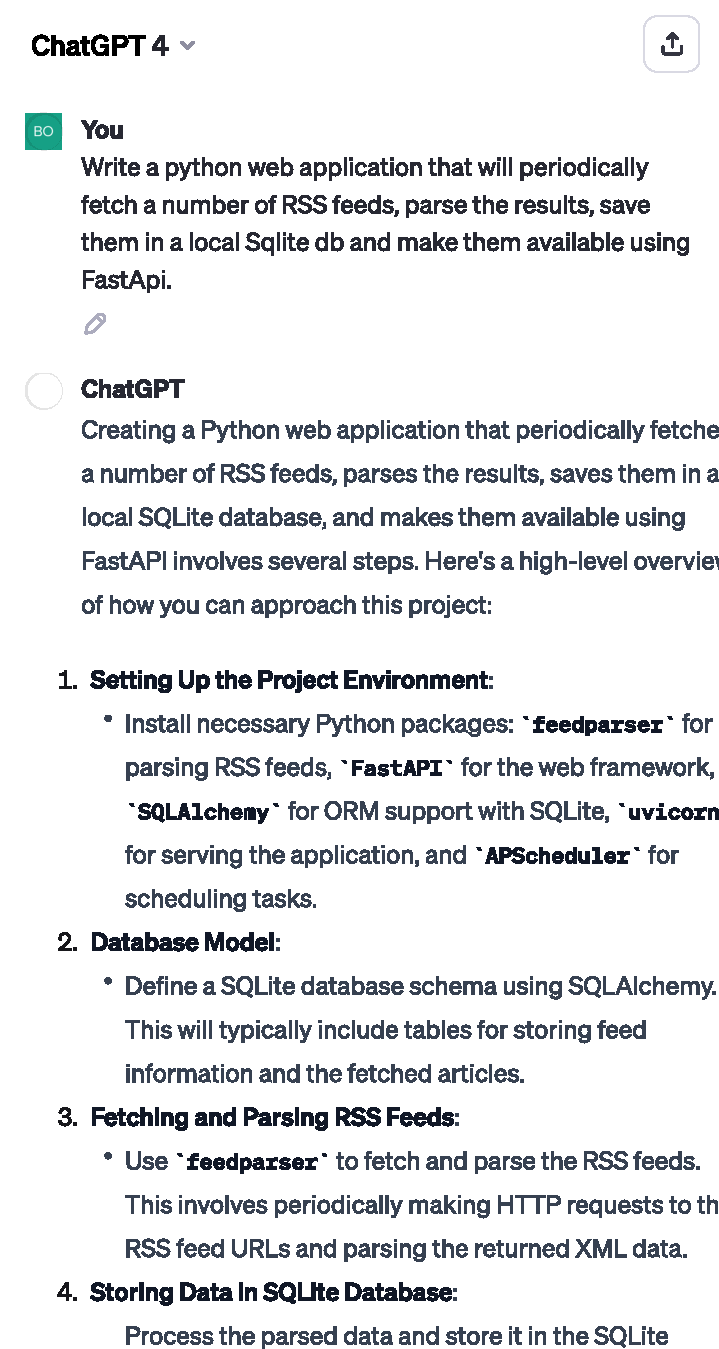
\includegraphics[width=0.65\textwidth]{prompt_2.pdf}
	\caption{Impelementációhoz prompt (nem teljes válasz)}{Ez a prompt persze nem produkált elsőre tökéletesen műdödő szoftvert, bőven volt mit kiegészíteni.}
\end{figure}

Az elkészült projekt \texttt{feedparser}-t alkalmaz az RSS/Atom feed-ek elemzéséhez, \texttt{FastAPI}-t a webes keretrendszerhez, \texttt{SQLAlchemy}-t az ORM támogatáshoz SQLite-al, \texttt{uvicorn}-t az alkalmazás szolgáltatásához, és \texttt{APScheduler}-t az időzített feladatokhoz.

A szoftver ki lett egészítve egy funkcióval a duplikált cikkek kezelésére, amely magában foglalja az egyedi cím és link kombinációk ellenőrzését az adatbázisban, mielőtt azokat hozzáadná. A \texttt{feedparser} által visszaadott \texttt{published\_parsed} dátumokat \texttt{datetime} objektummá alakítottuk, hogy kompatibilisek legyenek az SQLite \texttt{DateTime} típusával.

A programot továbá úgy módosítottam, hogy az rss feedek listáját egy yaml fájlból olvassa be.

\subsection{Részletesebb adatok parsolása}

Az eddigi megoldást még ki akartam egészíteni azzal, hogy a cikkek teljes szövegét letöltöm, ami alapból nem szokott az RSS/Atom folyamban eltárolva lenni. Ezt törvényeket betartva \texttt{robots.txt} értelmezése mellet végeztem. Mivel a cikkek szövege minden oldal esetében más html szerkezetben található ezt is a konfig fájlba tettem a feed url mellé. Eredetileg a ChatGPT-t szerettem volna rávenni, hogy a css selectorokat megírja, de a html dokumentumok értelmezése sok volt neki.

\section{Eredmény}

A szoftver három endpointon elérhető:
\begin{itemize}
	\item \texttt{/feeds/}: minden lehetséges feed
	\item \texttt{/articles/}: minden cikk
	\item \texttt{/articles/\{feed\}}: minden cikk az adott feed-ben
\end{itemize}

Indítás: \texttt{uvicorn main:app --reload}\\

Használat példák (direkt rövidítve):\\

\begin{verbatim}
$ curl http://127.0.0.1:8000/feeds/

["24.hu","444.hu","atlatszo.hu","g7.hu","hang.hu","index.hu","magyarnarancs.hu","mfor.hu",
 "nepszava.hu","telex.hu","rtl.hu","szabadeuropa.hu","valaszonline.hu","origo.hu",
 "pestisracok.hu","mandiner.hu","baon.hu","bama.hu","beol.hu","magyarnemzet.hu","hirtv.hu",
 "vg.hu","figyelo.hu","oroszhirek.hu","kuruc.info","magyarjelen.hu"]

$ curl http://127.0.0.1:8000/articles/

[{"published":"2023-11-28T15:34:41","id":1,"content":"A Fővárosi Törvényszék ...",
  "link":"https://telex.hu/belfold/2023/11/28/fegyhaz-taxi-buszsofor","feed":"telex.hu",
  "title":"Fegyházbüntetést kapott a taxisofőr, aki rátámadt egy buszsofőrre"}, ...]

$ curl http://127.0.0.1:8000/articles/24.hu

[{"published":"2023-11-28T15:22:02","id":11,"content":"Úgy látszik, véget nem érő ...",
  "link":"https://24.hu/szorakozas/2023/11/28/sztarbox-2023-racz-jeno-istenes-bence-ring-beszolas/",
  "feed":"24.hu","title":"Istenes Bence: A cigányozás miben más, mint a buzizás a ringben?"}, ...]
\end{verbatim}

\section{Verziókövetés}

A megoldás és a dokumentáció forráskódja a következő git repository-ban elérhető: \url{https://github.com/boapps/hu-news-scraper}

\end{document}
